\noindent
Por último, se realizó una predicción con el algoritmo de Holt Winters. El proceso que se debe seguir para realizar dicha predicción es similar al utilizado con el algoritmo de mínimos cuadrados, pero la gran diferencia radica en que ahora almacenaremos distintas colecciones de datos para poder realizar la predicción. En la siguiente imagen se muestra la nueva estructura del archivo .rrd.
\newline
Finalmente, tras recolectar datos de nuestro dispositivo durante un breve periodo de tiempo, es posible ir calculando una predicción, la cual a su vez posee límites superiores e inferiores que nos indican la variación máxima que está permitida para el recurso que se está monitoreando. La siguiente imagen muestra la forma en que se realiza la creación de la gráfica, así como una gráfica de muestra generada.

\begin{figure}[htbp!]
	\centering
		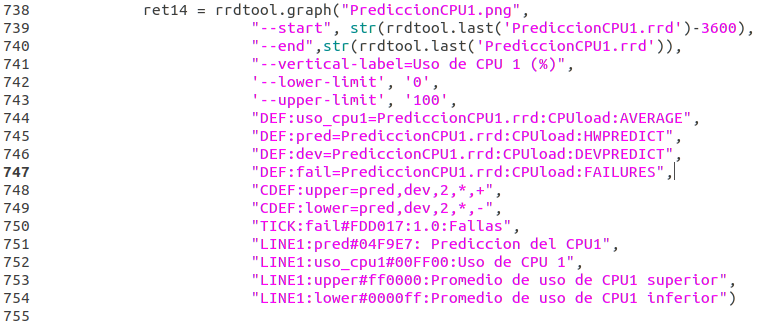
\includegraphics[width=0.8\textwidth]{imagenes/HoltWinters/CreacionImagenHoltWinters.png}
	\caption{Aplicación del algoritmo de Holt Winters para crear la gráfica de la predicción.}
\end{figure}

\begin{figure}[htbp!]
	\centering
		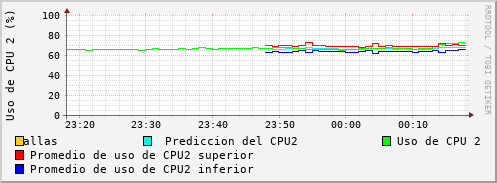
\includegraphics[width=0.8\textwidth]{imagenes/HoltWinters/PrediccionCPU2.png}
	\caption{Predicción para el uso del CPU 2.}
\end{figure}

\begin{figure}[htbp!]
	\centering
		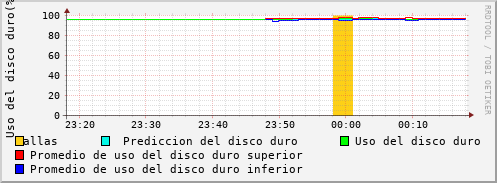
\includegraphics[width=0.8\textwidth]{imagenes/HoltWinters/PrediccionDisco.png}
	\caption{Predicción para el uso del disco duro.}
\end{figure}

\begin{figure}[htbp!]
	\centering
		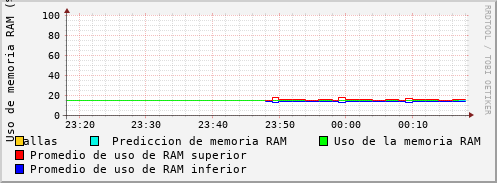
\includegraphics[width=0.8\textwidth]{imagenes/HoltWinters/PrediccionRAM.png}
	\caption{Predicción para el uso de la memoria RAM.}
\end{figure}

